\documentclass[9pt,pdf,hyperref={unicode}]{beamer}
\beamertemplatenavigationsymbolsempty

\setbeamertemplate{blocks}[rounded=true, shadow=true]
\setbeamertemplate{footline}[page number]
\usepackage{multicol}

\usefonttheme{serif}

\usepackage[utf8]{inputenc}
\usepackage[english, russian]{babel}
\usepackage{amsmath,mathrsfs,mathtext}
\usepackage{graphicx, epsfig}
\usepackage{caption}
\usepackage{subfig}
\usepackage{amsmath, bm}

\usepackage{comment}

\usepackage{tabularx}

\usepackage{tikz}

\DeclareMathOperator*{\argmin}{arg\,min}
\DeclareMathOperator*{\argmax}{arg\,max}

\makeatletter
\let\@@magyar@captionfix\relax
\makeatother

\usetheme{Warsaw}
\usecolortheme{sidebartab}
\definecolor{beamer@blendedblue}{RGB}{31,96,49}

\setbeamertemplate{enumerate items}[circle]

\setbeamersize{text margin left=1.5em, text margin right=1.5em}

\usepackage{ragged2e}

\usepackage{etoolbox}% http://ctan.org/pkg/etoolbox
\AtBeginEnvironment{figure}{\setcounter{subfigure}{0}}% Resets subfigure counter at start of figure environment

%----------------------------------------------------------------------------------------------------------
\title[\hbox to 56mm{Смесь экспертов \hfill\insertframenumber\,/\,\inserttotalframenumber}]
{Смесь экспертов}
\author[Грабовой А.\ В.]{\Large Грабовой Андрей Валериевич}
\institute{ Московский физико-технический институт\\
Факультет управления и прикладной математики\\
Кафедра интеллектуальных систем\\
}
\date{\footnotesize{\emph{Москва}\\
 2019 г}}
%----------------------------------------------------------------------------------------------------------
\begin{document}
%----------------------------------------------------------------------------------------------------------
\begin{frame}
\titlepage
\end{frame}

%----------------------------------------------------------------------------------------------------------
\begin{frame}{План}
	\begin{enumerate}
		\item ЕМ--алгоритм:
			\begin{itemize}
				\item Классический,
				\item Вариационный,
			\end{itemize}
		\item Смесь моделей:
			\begin{itemize}
				\item Постановка задачи,
				\item Итерационные формулы полученные при помощи вариационного ЕМ--алгоритма,
				\item Илюстрация сходимости,
			\end{itemize}
		\item Смесь экспертов
			\begin{itemize}
				\item Постановка задачи,
				\item Итерационные формулы полученные при помощи вариационного ЕМ--алгоритма,
				\item Илюстрация сходимости,
			\end{itemize}
	\end{enumerate}
\end{frame}
%----------------------------------------------------------------------------------------------------------
\begin{frame}{Вариационный ЕМ--алгоритм}
\justifying
	Максимизация обоснованости:
	\begin{equation}
	\label{sl:1:eq:1}
		\begin{aligned}
			\bm{\Theta} = \arg\max_{\bm{\Theta}} p\left(\textbf{y}|\textbf{X}, \bm{\Theta}\right)
		\end{aligned}
	\end{equation}
	ELBO:
	\begin{equation}
	\label{sl:1:eq:2}
		\begin{aligned}
			\mathcal{L}\left(q\bigr(\textbf{Z}\bigr), \bm{\Theta}\right)&= \int q\bigr(\textbf{Z}\bigr)\log\frac{p\left(\textbf{y}, \textbf{Z}|\bm{\Theta}, \textbf{X}\right)}{q\left(\textbf{Z}\right)}d\textbf{Z}\\
			&=p\left(\textbf{y}|\textbf{X}, \bm{\Theta}\right) - \mathsf{D}_{KL}\left(q\bigr(\textbf{Z}\bigr)||p\bigr(\textbf{Z}|\textbf{y}, \textbf{X}, \bm{\Theta}\bigr)\right)
		\end{aligned}
	\end{equation}
	ЕМ--алгоритм:
	\begin{enumerate}
		\item Е--шаг: 
			\begin{equation}
			\label{sl:1:eq:3}
				\begin{aligned}
					q^{s}\bigr(\textbf{Z}\bigr) = \arg\max_{q\bigr(\textbf{Z}\bigr)\in Q} \mathcal{L}\left(q\bigr(\textbf{Z}\bigr), \bm{\Theta}^{s-1}\right)		
				\end{aligned}
			\end{equation}
		\item М--шаг: 
			\begin{equation}
			\label{sl:1:eq:4}
				\begin{aligned}
					\bm{\Theta}^{s} = \arg\max_{\bm{\Theta}} \mathcal{L}\left(q^{s}\bigr(\textbf{Z}\bigr), \bm{\Theta}\right)		
				\end{aligned}
			\end{equation}
	\end{enumerate}
	
	Вариационный ЕМ--алгоритм (Mean Field Approximation\footnote[1]{\url{https://github.com/andriygav/EMprior/blob/master/Lecture/Grabovoy2019MeanField.pdf}}):
	\begin{enumerate}
		\item Е--шаг: 
			\begin{equation}
			\label{sl:1:eq:5}
				\begin{aligned}
					\log q\left(\textbf{Z}_{k}^{s}\right) \propto \mathsf{E}_{q/k}\log p\left(\textbf{y}, \textbf{Z}|\textbf{X},\bm{\Theta}^{s-1}\right)
				\end{aligned}
			\end{equation}
		\item М--шаг: 
			\begin{equation}
			\label{sl:1:eq:6}
				\begin{aligned}
					\bm{\Theta}^{s} = \arg\max_{\bm{\Theta}} \mathbf{E}_{q^{s}}\log p\left(\textbf{y}, \textbf{Z}|\textbf{X},\bm{\Theta}\right)
				\end{aligned}
			\end{equation}
	\end{enumerate}

\end{frame}
%----------------------------------------------------------------------------------------------------------
\begin{frame}{Смесь моделей}
\justifying
\begin{definition}
Смесь моделей~---~мультимодель, ответы которой представляют собой взвешенную сумму ответов всех задействованных моделей независимо от объекта.

\begin{equation}
\label{sl:2:eq:1}
	\begin{aligned}
		\hat{\textbf{f}} = \sum_{k=1}^{K}\pi_{k}\textbf{f}_k, \qquad \pi_{k} = const, \quad \sum_{k=1}^{K}\pi_{k} = 1,
	\end{aligned}
\end{equation}
где~$\textbf{f}$~---~мультимодель, а $\textbf{f}_k$~---~локальная модель.
\end{definition}

{\bf Пример 1}:
\begin{enumerate}
	\item Веса моделей в смеси~$\bm{\pi}$ получены из априорного распределения 
		\begin{equation}
		\label{sl:2:eq:2}
			\begin{aligned}
				p\left(\bm{\pi}|\mu\right);
			\end{aligned}
		\end{equation}
	\item Вектора параметров~$\textbf{w}_k$ получены из нормального распределения 
		\begin{equation}
		\label{sl:2:eq:3}
			\begin{aligned}
				p\left(\textbf{w}_k|\textbf{A}_k\right) = \mathcal{N}\left(\textbf{w}_k|\textbf{0}, \textbf{A}_{k}\right),~k=1,\cdots K;
			\end{aligned}
		\end{equation}
		
	\item Для каждого объекта~$\textbf{x}_i$ существует модель~$\textbf{f}_{k_i},$ которой он описывается, причем $p\left(k_i=k\right) = \pi_k;$
	
	\item  Для каждого объекта $\textbf{x}_i$ класс $y_i$ определен в соответсвии с моделью 
		\begin{equation}
		\label{sl:2:eq:3}
			\begin{aligned}
				\textbf{f}_{k_i}:~y_i\sim~\mathcal{N}\left(\textbf{w}_{k_i}^{\mathsf{T}}\textbf{x}_i + b_k, \beta^{-1}\right)
			\end{aligned}
		\end{equation}
\end{enumerate}

\end{frame}
%----------------------------------------------------------------------------------------------------------
\begin{frame}{Пример 1}
\justifying
Правдоподобие модели:
	\begin{equation}
	\label{sl:3:eq:1}
		\begin{aligned}
			p(\textbf{y}, \textbf{W}, \bm{\pi}|\textbf{X}, \textbf{A}, \beta, \bm{\mu}) = \text{Dir}(\bm{\pi}|\bm{\mu})
			\prod_{k=1}^{K}N(\textbf{w}_k|\textbf{0}, \textbf{A}_k)
			\prod_{i=1}^{N}\left(\sum_{k=1}^{K}\pi_k\mathcal{N}(y_i|\textbf{w}_k^{\mathsf{T}}\textbf{x}_i, \beta^{-1})\right)
		\end{aligned}
	\end{equation}
Введем скрытые переменные $\textbf{Z} = ||z_{ik}||,$ где $~z_{ik} = 1 \Leftrightarrow k_i=k$:
	\begin{equation}
	\label{sl:3:eq:2}
		\begin{aligned}
			p(\textbf{y}, \textbf{W}, \bm{\pi}, \textbf{Z}|\textbf{X}, \textbf{A}, \beta, \bm{\mu}) = \text{Dir}(\bm{\pi}|\bm{\mu})
			\prod_{k=1}^{K}N(\textbf{w}_k|\textbf{0}, \textbf{A}_k)
			\prod_{i=1}^{N}\prod_{k=1}^{K}\left(\pi_k\mathcal{N}(y_i|\textbf{w}_k^{\mathsf{T}}\textbf{x}_i, \beta^{-1})\right)^{z_{ik}}
		\end{aligned}
	\end{equation}

Вариационный ЕМ--алгоритм $q\left(\textbf{Z}, \textbf{W}, \bm{\pi}\right) = q\left(\textbf{Z}\right)q\left(\textbf{W}\right)q\left(\bm{\pi}\right)$:
	\begin{enumerate}
		\item Е--шаг: 
			\begin{equation}
			\label{sl:3:eq:3}
				\begin{aligned}
					\log q\left(\textbf{Z}^{s}\right) &\propto \mathsf{E}_{q/\textbf{Z}}\log p(\textbf{y}, \textbf{W}, \bm{\pi}, \textbf{Z}|\textbf{X}, \textbf{A}^{s-1}, \beta^{s-1}, \bm{\mu})\\
					\log q\left(\textbf{W}^{s}\right) &\propto \mathsf{E}_{q/\textbf{W}}\log p(\textbf{y}, \textbf{W}, \bm{\pi}, \textbf{Z}|\textbf{X}, \textbf{A}^{s-1}, \beta^{s-1}, \bm{\mu})\\
					\log q\left(\bm{\pi}^{s}\right) &\propto \mathsf{E}_{q/\bm{\pi}}\log p(\textbf{y}, \textbf{W}, \bm{\pi}, \textbf{Z}|\textbf{X}, \textbf{A}^{s-1}, \beta^{s-1}, \bm{\mu})\\
				\end{aligned}
			\end{equation}
		\item М--шаг: 
			\begin{equation}
			\label{sl:3:eq:4}
				\begin{aligned}
					\textbf{A}^{s}, \beta^{s} = \arg\max_{\textbf{A}, \beta} \mathbf{E}_{q^{s}}\log p(\textbf{y}, \textbf{W}, \bm{\pi}, \textbf{Z}|\textbf{X}, \textbf{A}, \beta, \bm{\mu})
				\end{aligned}
			\end{equation}
	\end{enumerate}

\end{frame}
%----------------------------------------------------------------------------------------------------------
\begin{frame}{Пример 1}
\justifying
Итерационные формулы ЕМ--алгоритма\footnote[1]{\url{https://github.com/andriygav/EMprior/blob/master/paper/Grabovoy2019Draft.pdf}}:
	\begin{enumerate}
		\item Е--шаг: 
			\begin{equation}
			\label{sl:4:eq:1}
				\begin{aligned}
					&p(z_{ik} = 1) = \frac{\exp\left(\mathsf{E}\log\pi_k - \frac{\beta}{2}\left[y_i^2 -2y_i\textbf{x}_i^{\mathsf{T}}\mathsf{E}\textbf{w}_k +\textbf{x}_i^{\mathsf{T}}\left(\mathsf{E}\textbf{w}_k\textbf{w}_k^{\mathsf{T}}\right)\textbf{x}_i\right] \right)}{\sum_k p(z_{ik}=1)},\\
					&q(\bm{\pi}) = \text{Dir}(\bm{\pi}|\bm{\mu}+ \bm{\gamma}), \quad
					q(\textbf{w}_k) = \mathcal{N}(\textbf{w}_k|\textbf{m}_k, \textbf{B}_k),\\
					&\gamma_k=\sum_{i=1}^{N}\mathsf{E}z_{ik}, \quad 
					\textbf{m}_k = \beta\textbf{B}_k\left(\sum_{i=1}^{N}\textbf{x}_iy_i\mathsf{E}z_{ik} \right), \quad
					\textbf{B}_k = \left(\textbf{A}_k^{-1} + \beta\sum_{i=1}^{N}\textbf{x}_i\textbf{x}_i^{\mathsf{T}}\mathsf{E}z_{ik}\right)^{-1}.
				\end{aligned}
			\end{equation}
		\item М--шаг: 
			\begin{equation}
			\label{sl:4:eq:2}
				\begin{aligned}
					\textbf{A}_k &= \mathsf{E}\textbf{w}_k\textbf{w}_k^{\mathsf{T}}\\
					 \frac{1}{\beta} &= \frac{\sum\sum\left[y_i^2 -2y_i\textbf{x}_i^{\mathsf{T}}\mathsf{E}\textbf{w}_k+\textbf{x}_i^{\mathsf{T}}\mathsf{E}\textbf{w}_k\textbf{w}_k^{\mathsf{T}}\textbf{x}_i\right]\mathsf{E}z_{ik}}{\sum\sum \mathsf{E}z_{ik}}
				\end{aligned}
			\end{equation}
	\end{enumerate}
Некоторые математические ожидания:
	\begin{enumerate}
		\item $\mathsf{E}z_{ik} = p(z_{ik} = 1),$
		\item $\mathsf{E}\log\pi_{k} = \psi^{0}(\mu_k + \gamma_k) - \psi^{0}(K\mu_k + N),$
		\item $\mathsf{E}\textbf{w}_k\textbf{w}_k^{\mathsf{T}} = \textbf{B}_k + \textbf{m}_k\textbf{m}_k^{\mathsf{T}}.$
	\end{enumerate}
\end{frame}
%----------------------------------------------------------------------------------------------------------
\begin{frame}{Пример 1}
\justifying
\begin{figure}
	\subfloat[]{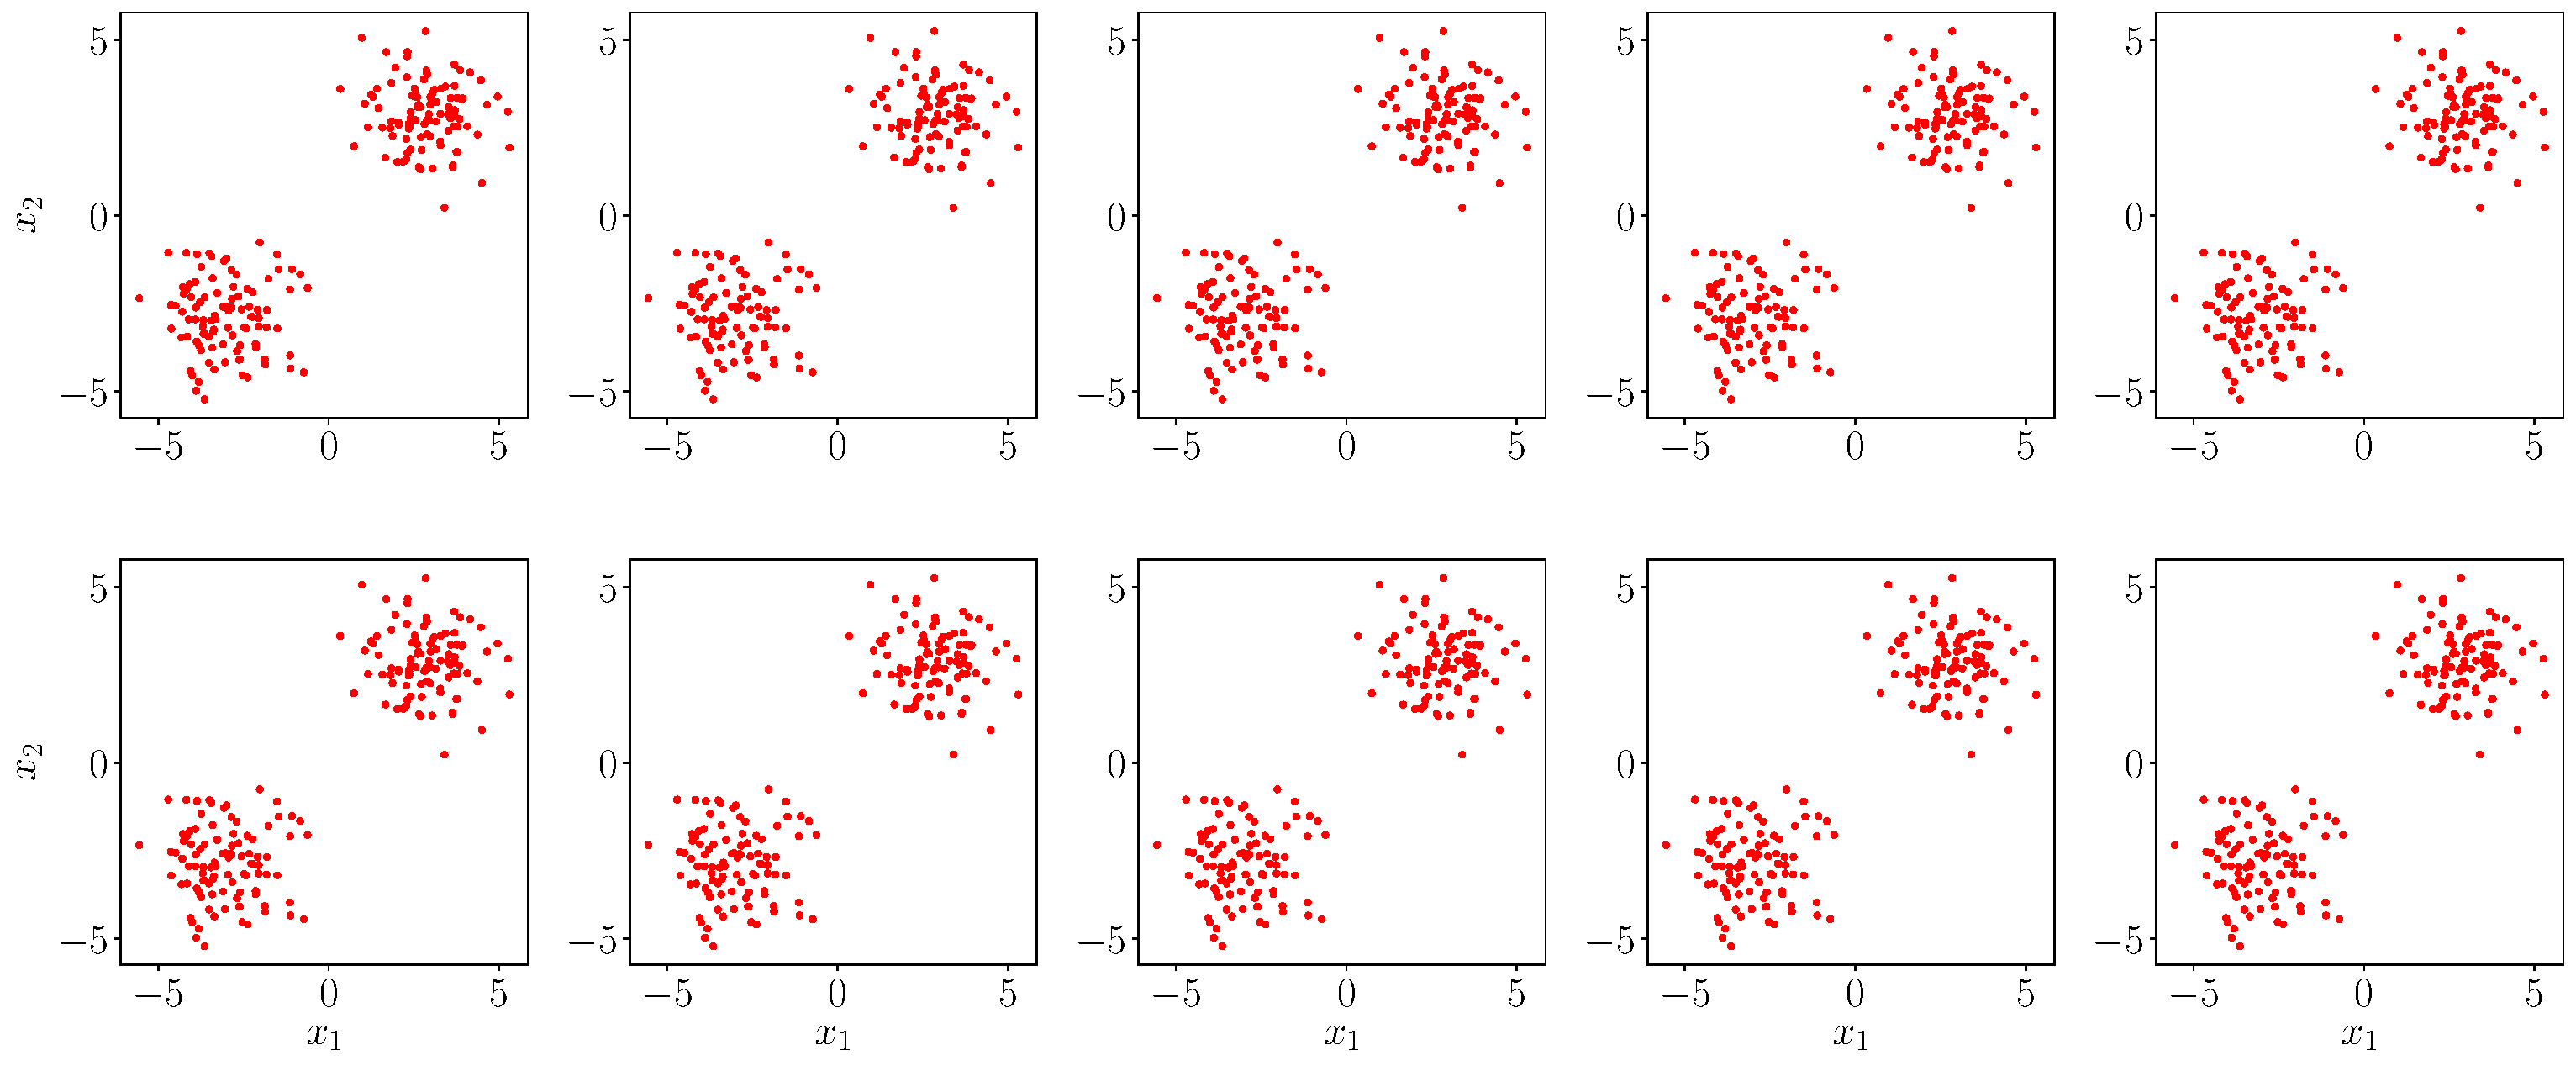
\includegraphics[height=0.35\textheight]{pictures/pi_predicftion_models}\label{sl:8:pic:1}}
	\subfloat[]{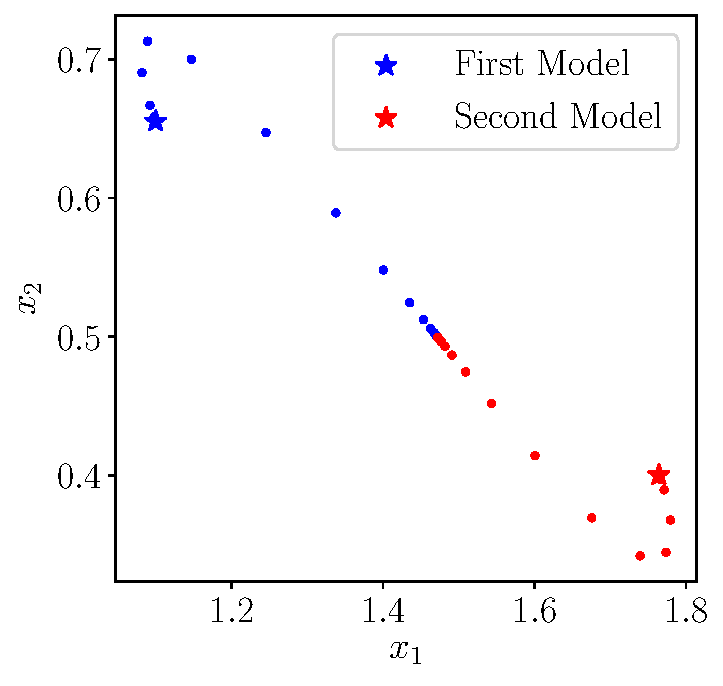
\includegraphics[height=0.35\textheight]{pictures/parameters_models}\label{sl:8:pic:2}}
\end{figure}
На рис.~\ref{sl:8:pic:1} показано, что в случае смеси моделей, предсказать то, какую модель использовать в каждой точке нельзя.

На рис.~\ref{sl:8:pic:2} показана зависимость векторов $\mathbf{w}_{k}$~---~параметры локальных моделей в процессе обучения.

\footnotetext[1]{\url{https://github.com/andriygav/MixtureLib}}
\end{frame}
%----------------------------------------------------------------------------------------------------------
\begin{frame}{Смесь экспертов}
\justifying
\begin{definition}
\label{sl:5:eq:1}
Смесь экспертов~---~мультимодель, определяющая правдоподобие веса $\pi_k$ каждой локальной модели $\textbf{f}_k$ на признаковом описании объекта $\textbf{x}$.

\begin{equation}
\label{sl:5:eq:2}
\begin{aligned}
\hat{\mathbf{f}} = \sum_{k=1}^{K}\pi_{k}\mathbf{f}_k, \qquad \pi_{k}\left(\mathbf{x}, \mathbf{V}\right):\mathbb{R}^{n\times \left|\mathbf{V}\right|} \to [0, 1], \qquad \sum_{k=1}^{K}\pi_{k}\left(\mathbf{x}, \mathbf{V}\right) = 1
\end{aligned}
\end{equation}
где~$\hat{\mathbf{f}}$~---~мультимодель, а $\mathbf{f}_k$ является некоторой моделью, $\pi_k$~---~параметрическая модель, $\mathbf{w}_k$~---~параметры $k$-й локальной модели, $\mathbf{V}$~---~параметры шлюзовой функции.
\end{definition}
{\bf Пример 2}:
	\begin{enumerate}
		\item Правдоподобие $k$-й локальной модели $p_{k}\left(y_{i}|\mathbf{w}_{k}, \mathbf{x}_{i}\right) = \mathcal{N}\left(y_{i}|\mathbf{w}_{k}^{\mathsf{T}}\mathbf{x}_{i}, \beta^{-1}\right),$
		\item Априорное распределение параметров $k$-й локальной модели $p^{k}\left(\mathbf{w}_{k}\right) = \mathcal{N}\left(\mathbf{w}_{k}|\mathbf{w}^{0}_{k}, \mathbf{A}_{k}\right),$
		\item Шлюзовая функция $\bm{\pi}\left(\mathbf{x}, \mathbf{V}\right) = \text{softmax}\bigr(\mathbf{V}_{1}^{\mathsf{T}}\bm{\sigma}\left(\mathbf{V}_2^{\mathsf{T}}\mathbf{x}\right)\bigr).$
	\end{enumerate}
\end{frame}
%----------------------------------------------------------------------------------------------------------
\begin{frame}{Пример 2}
\justifying
Правдоподобие модели:
	\begin{equation}
	\label{sl:6:eq:1}
		\begin{aligned}
			p\bigr(\mathbf{y}, \mathbf{W}|\mathbf{X}, \mathbf{V}, \textbf{A}, \textbf{W}^{0}, \beta\bigr) = \prod_{k=1}^{K}\mathcal{N}\left(\mathbf{w}_{k}|\mathbf{w}^{0}_{k}, \mathbf{A}_{k}\right)\prod_{i=1}^{N}\left(\sum_{k=1}^{K}\pi_{k}\mathcal{N}\left(y_{i}|\mathbf{w}_{k}^{\mathsf{T}}\mathbf{x}_{i}, \beta^{-1}\right)\right).
		\end{aligned}
	\end{equation}
Введем скрытые переменные $\textbf{Z} = ||z_{ik}||,$ где $~z_{ik} = 1 \Leftrightarrow k_i=k$:
	\begin{equation}
	\label{sl:6:eq:2}
		\begin{aligned}
			p\bigr(\mathbf{y}, \textbf{Z}, \mathbf{W}|\mathbf{X}, \mathbf{V}, \textbf{A}, \textbf{W}^{0}, \beta\bigr) = \prod_{k=1}^{K}\mathcal{N}\left(\mathbf{w}_{k}|\mathbf{w}^{0}_{k}, \mathbf{A}_{k}\right)\prod_{i=1}^{N}\prod_{k=1}^{K}\left(\pi_{k}\mathcal{N}\left(y_{i}|\mathbf{w}_{k}^{\mathsf{T}}\mathbf{x}_{i}, \beta^{-1}\right)\right)^{z_{ik}}.		
		\end{aligned}
	\end{equation}
Вариационный ЕМ--алгоритм $q\left(\textbf{Z}, \textbf{W}\right) = q\left(\textbf{Z}\right)q\left(\textbf{W}\right)$:
	\begin{enumerate}
		\item Е--шаг: 
			\begin{equation}
			\label{sl:6:eq:3}
				\begin{aligned}
					\log q\left(\textbf{Z}^{s}\right) &\propto \mathsf{E}_{q/\textbf{Z}}\log p\bigr(\mathbf{y}, \textbf{Z},\mathbf{W}|\mathbf{X}, \mathbf{V}^{s-1}, \textbf{A}^{s-1}, \textbf{W}^{0, s-1}, \beta^{s-1}\bigr)\\
					\log q\left(\textbf{W}^{s}\right) &\propto \mathsf{E}_{q/\textbf{W}}\log p\bigr(\mathbf{y}, \textbf{Z},\mathbf{W}|\mathbf{X}, \mathbf{V}^{s-1}, \textbf{A}^{s-1}, \textbf{W}^{0, s-1}, \beta^{s-1}\bigr)
				\end{aligned}
			\end{equation}
		\item М--шаг: 
			\begin{equation}
			\label{sl:6:eq:4}
				\begin{aligned}
					\textbf{W}^{0, s}, \textbf{A}^{s}, \beta^{s} = \arg\max_{\textbf{W}^{0}, \textbf{A}, \beta} \mathbf{E}_{q^{s}}\log p\bigr(\mathbf{y}, \textbf{Z},\mathbf{W}|\mathbf{X}, \mathbf{V}, \textbf{A}, \textbf{W}^{0}, \beta\bigr)
				\end{aligned}
			\end{equation}
	\end{enumerate}
\end{frame}
%----------------------------------------------------------------------------------------------------------
\begin{frame}{Пример 2}
\justifying
Итерационные формулы ЕМ--алгоритма\footnote[1]{\url{https://github.com/andriygav/EMprior/blob/master/paper/Grabovoy2019MixtureOfExpert.pdf}}:
	\begin{enumerate}
		\item Е--шаг: 
			\begin{equation}
			\label{sl:7:eq:1}
				\begin{aligned}
					&p\left(z_{ik} = 1\right) = \frac{\exp\left(\log\pi_{k}\left(\textbf{x}_{i}, \textbf{V}\right) - \frac{\beta}{2}\left(\textbf{x}_{i}^{\mathsf{T}}\mathsf{E}\textbf{w}_{k}\textbf{w}_{k}^{\mathsf{T}}\textbf{x}_{i} - \textbf{x}_{i}^{\mathsf{T}}\mathsf{E}\textbf{w}_{k}\right)\right)}{\sum_{k'=1}^{K}\exp\left(\log\pi_{k'}\left(\textbf{x}_{i}, \textbf{V}\right) - \frac{\beta}{2}\left(\textbf{x}_{i}^{\mathsf{T}}\mathsf{E}\textbf{w}_{k'}\textbf{w}_{k'}^{\mathsf{T}}\textbf{x}_{i} - \textbf{x}_{i}^{\mathsf{T}}\mathsf{E}\textbf{w}_{k'}\right) \right)},\\
					&q(\textbf{w}_k) = \mathcal{N}(\textbf{w}_k|\textbf{m}_k, \textbf{B}_k),\\
					&\mathbf{m}_{k} = \mathbf{B}_{k}\left(\mathbf{A}_{k}^{-1}\mathbf{w}_{k}^{0}+\beta\sum_{i=1}^{N}\mathbf{x}_{i}y_{i}\mathsf{E}z_{ik}\right), \quad
					\mathbf{B}_{k} = \left(\mathbf{A}_{k}^{-1}+\beta\sum_{i=1}^{N}\mathbf{x}_{i}\mathbf{x}_{i}^{\mathsf{T}}\mathsf{E}z_{ik}\right)^{-1} .
				\end{aligned}
			\end{equation}
		\item М--шаг: 
			\begin{equation}
			\label{sl:7:eq:2}
				\begin{aligned}
					&\textbf{A}_{k} = \mathsf{E}\textbf{w}_{k}\textbf{w}_{k}^{\mathsf{T}} - \textbf{w}_{k}^{0}\mathsf{E}\textbf{w}_{k}^{\mathsf{T}} - \mathsf{E}\textbf{w}_{k}\textbf{w}_{k}^{0\mathsf{T}} + \textbf{w}_{k}^{0}\textbf{w}_{k}^{0\mathsf{T}}, \\
					 &\frac{1}{\beta}=\frac{1}{N}\sum_{i=1}^{N}\sum_{k=1}^{K}\left[y_{i}^{2}-2y_{i}\textbf{x}_{i}^{\mathsf{T}}\mathsf{E}\textbf{w}_{k} + \textbf{x}_{i}^{\mathsf{T}}\mathsf{E}\textbf{w}_{k}\textbf{w}_{k}^{\mathsf{T}}\textbf{x}_{i}\right]\mathsf{E}z_{ik},\\
					&\textbf{w}_{k}^{0} =\mathsf{E}\textbf{w}_{k},\\
					&\textbf{V}= \arg\max_{\textbf{V}} \mathbf{E}_{q^{s}}\log p\bigr(\mathbf{y}, \textbf{Z},\mathbf{W}|\mathbf{X}, \mathbf{V}, \textbf{A}, \textbf{W}^{0}, \beta\bigr).
				\end{aligned}
			\end{equation}
	\end{enumerate}
\end{frame}
%----------------------------------------------------------------------------------------------------------
\begin{frame}{Пример 2}
\justifying
\begin{figure}
	\subfloat[]{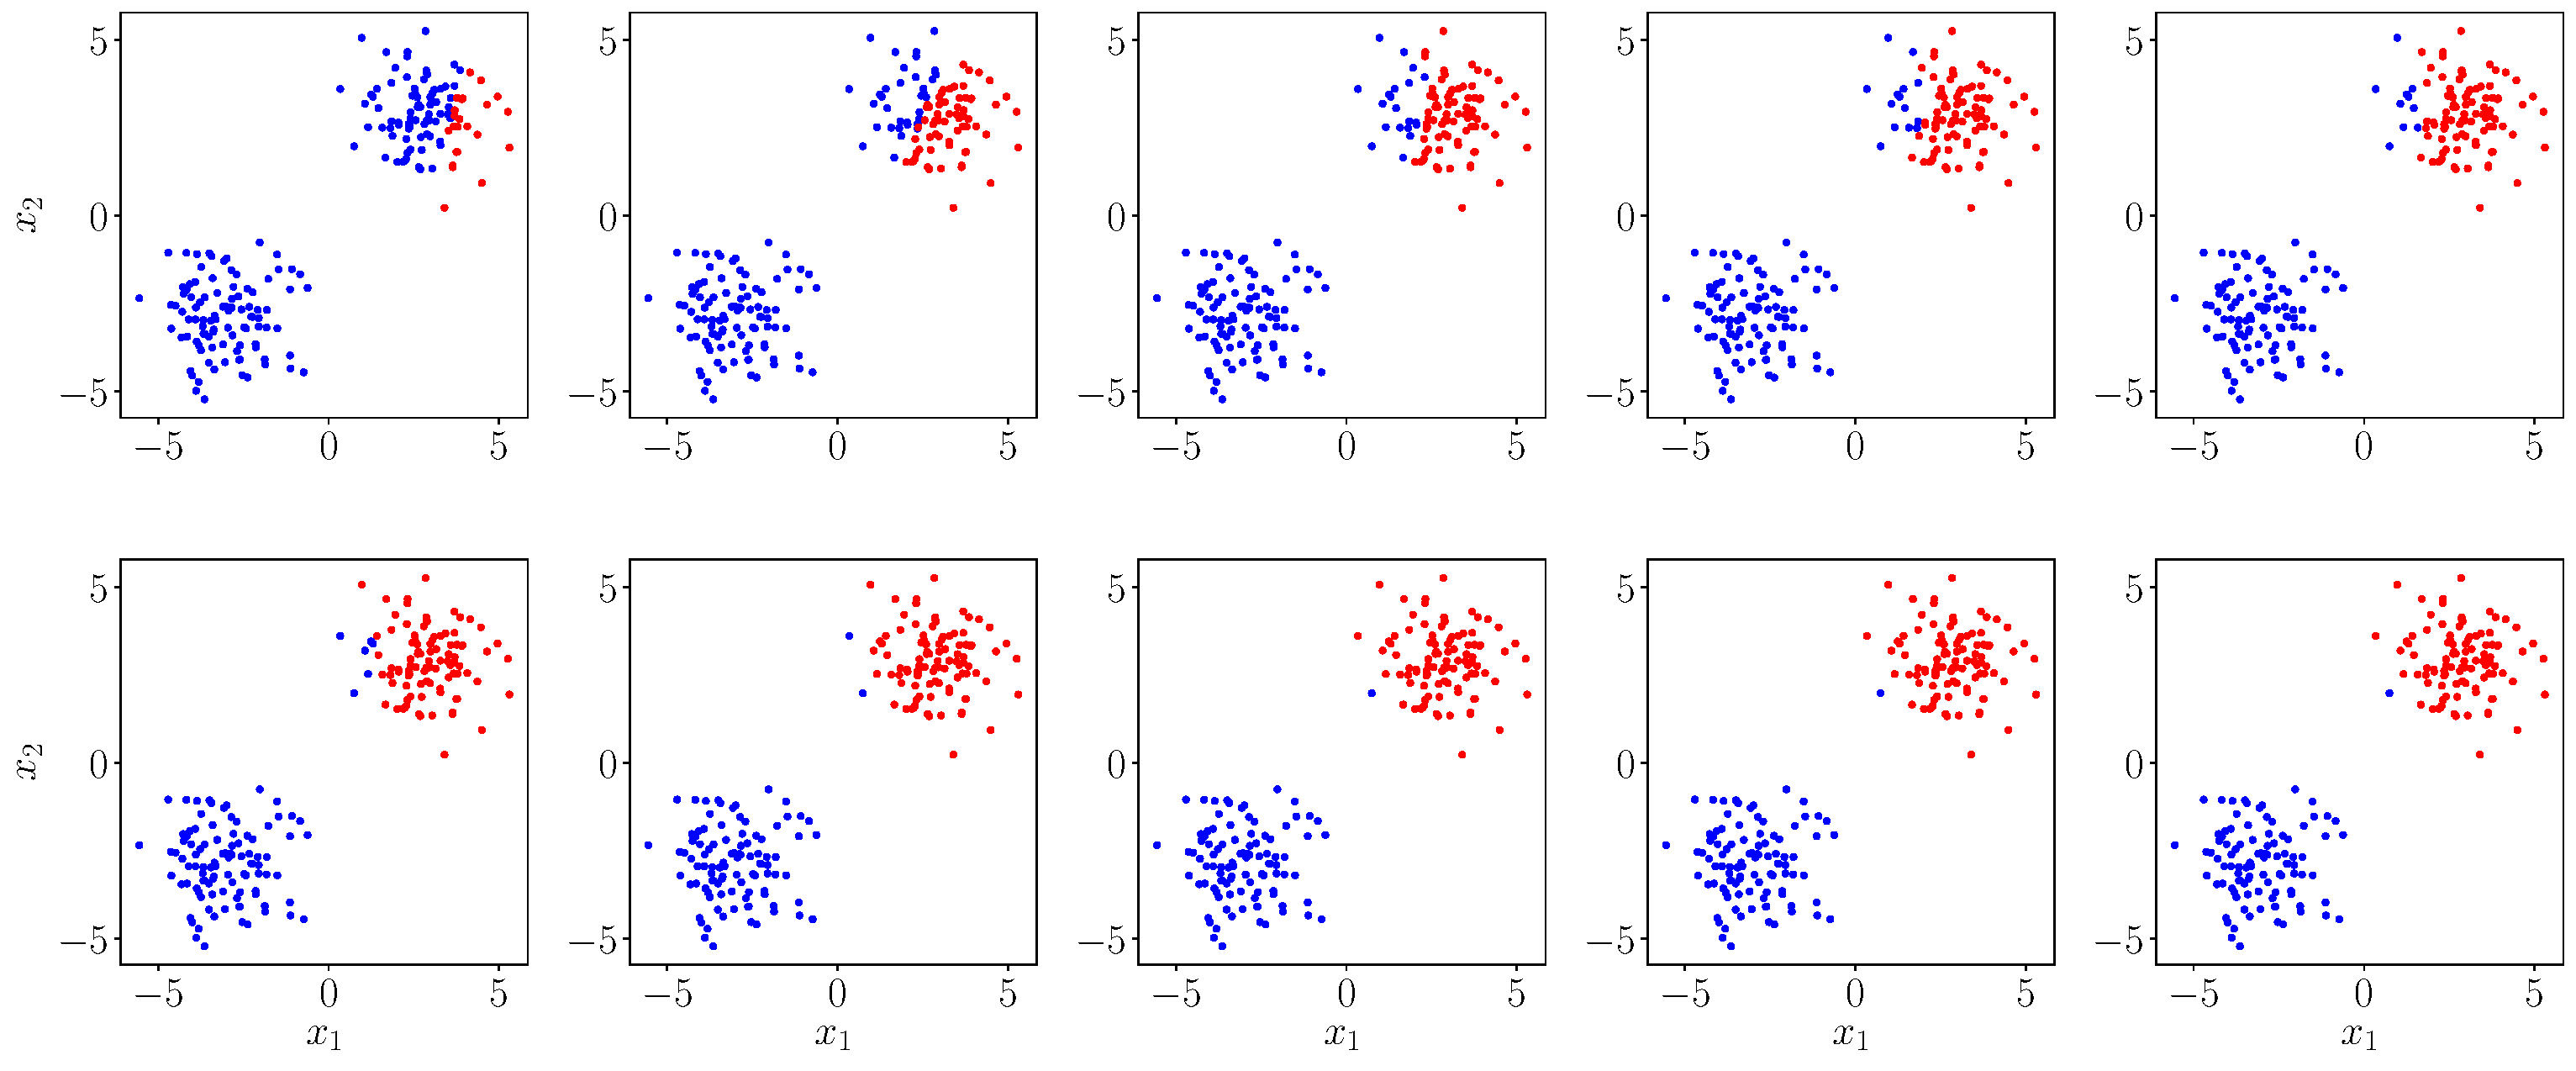
\includegraphics[height=0.35\textheight]{pictures/pi_predicftion_experts}\label{sl:9:pic:1}}
	\subfloat[]{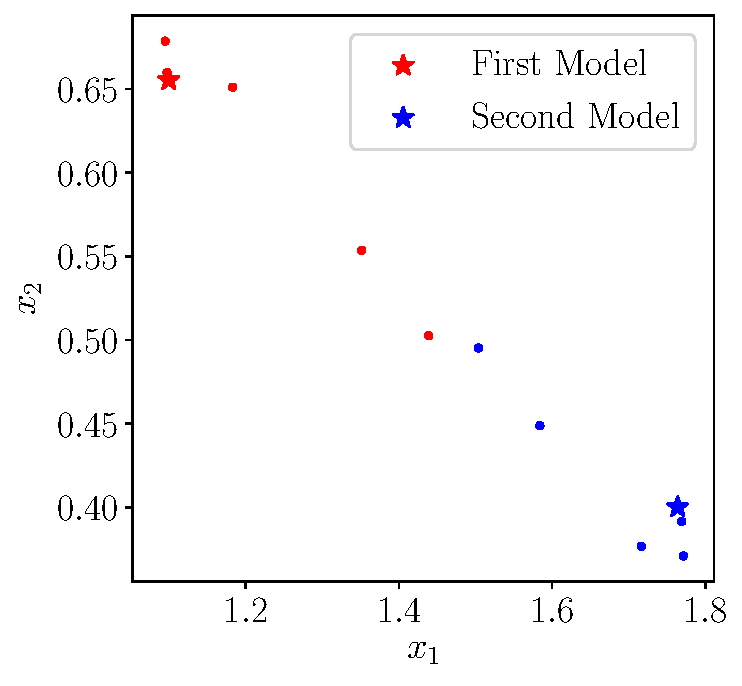
\includegraphics[height=0.35\textheight]{pictures/parameters_experts}\label{sl:9:pic:2}}
\end{figure}
На рис.~\ref{sl:9:pic:1} показано, что в случае смеси экспертов гипермодель предсказывает к какому классу относится каждая точка в пространстве объектов.

На рис.~\ref{sl:9:pic:2} показана зависимость векторов $\mathbf{w}_{k}$~---~параметры локальных моделей в процессе обучения.

\footnotetext[1]{\url{https://github.com/andriygav/MixtureLib}}
\end{frame}
%----------------------------------------------------------------------------------------------------------
\begin{frame}{Сравнение результатов}
\justifying
\begin{figure}
	\subfloat[Смесь Моделей]{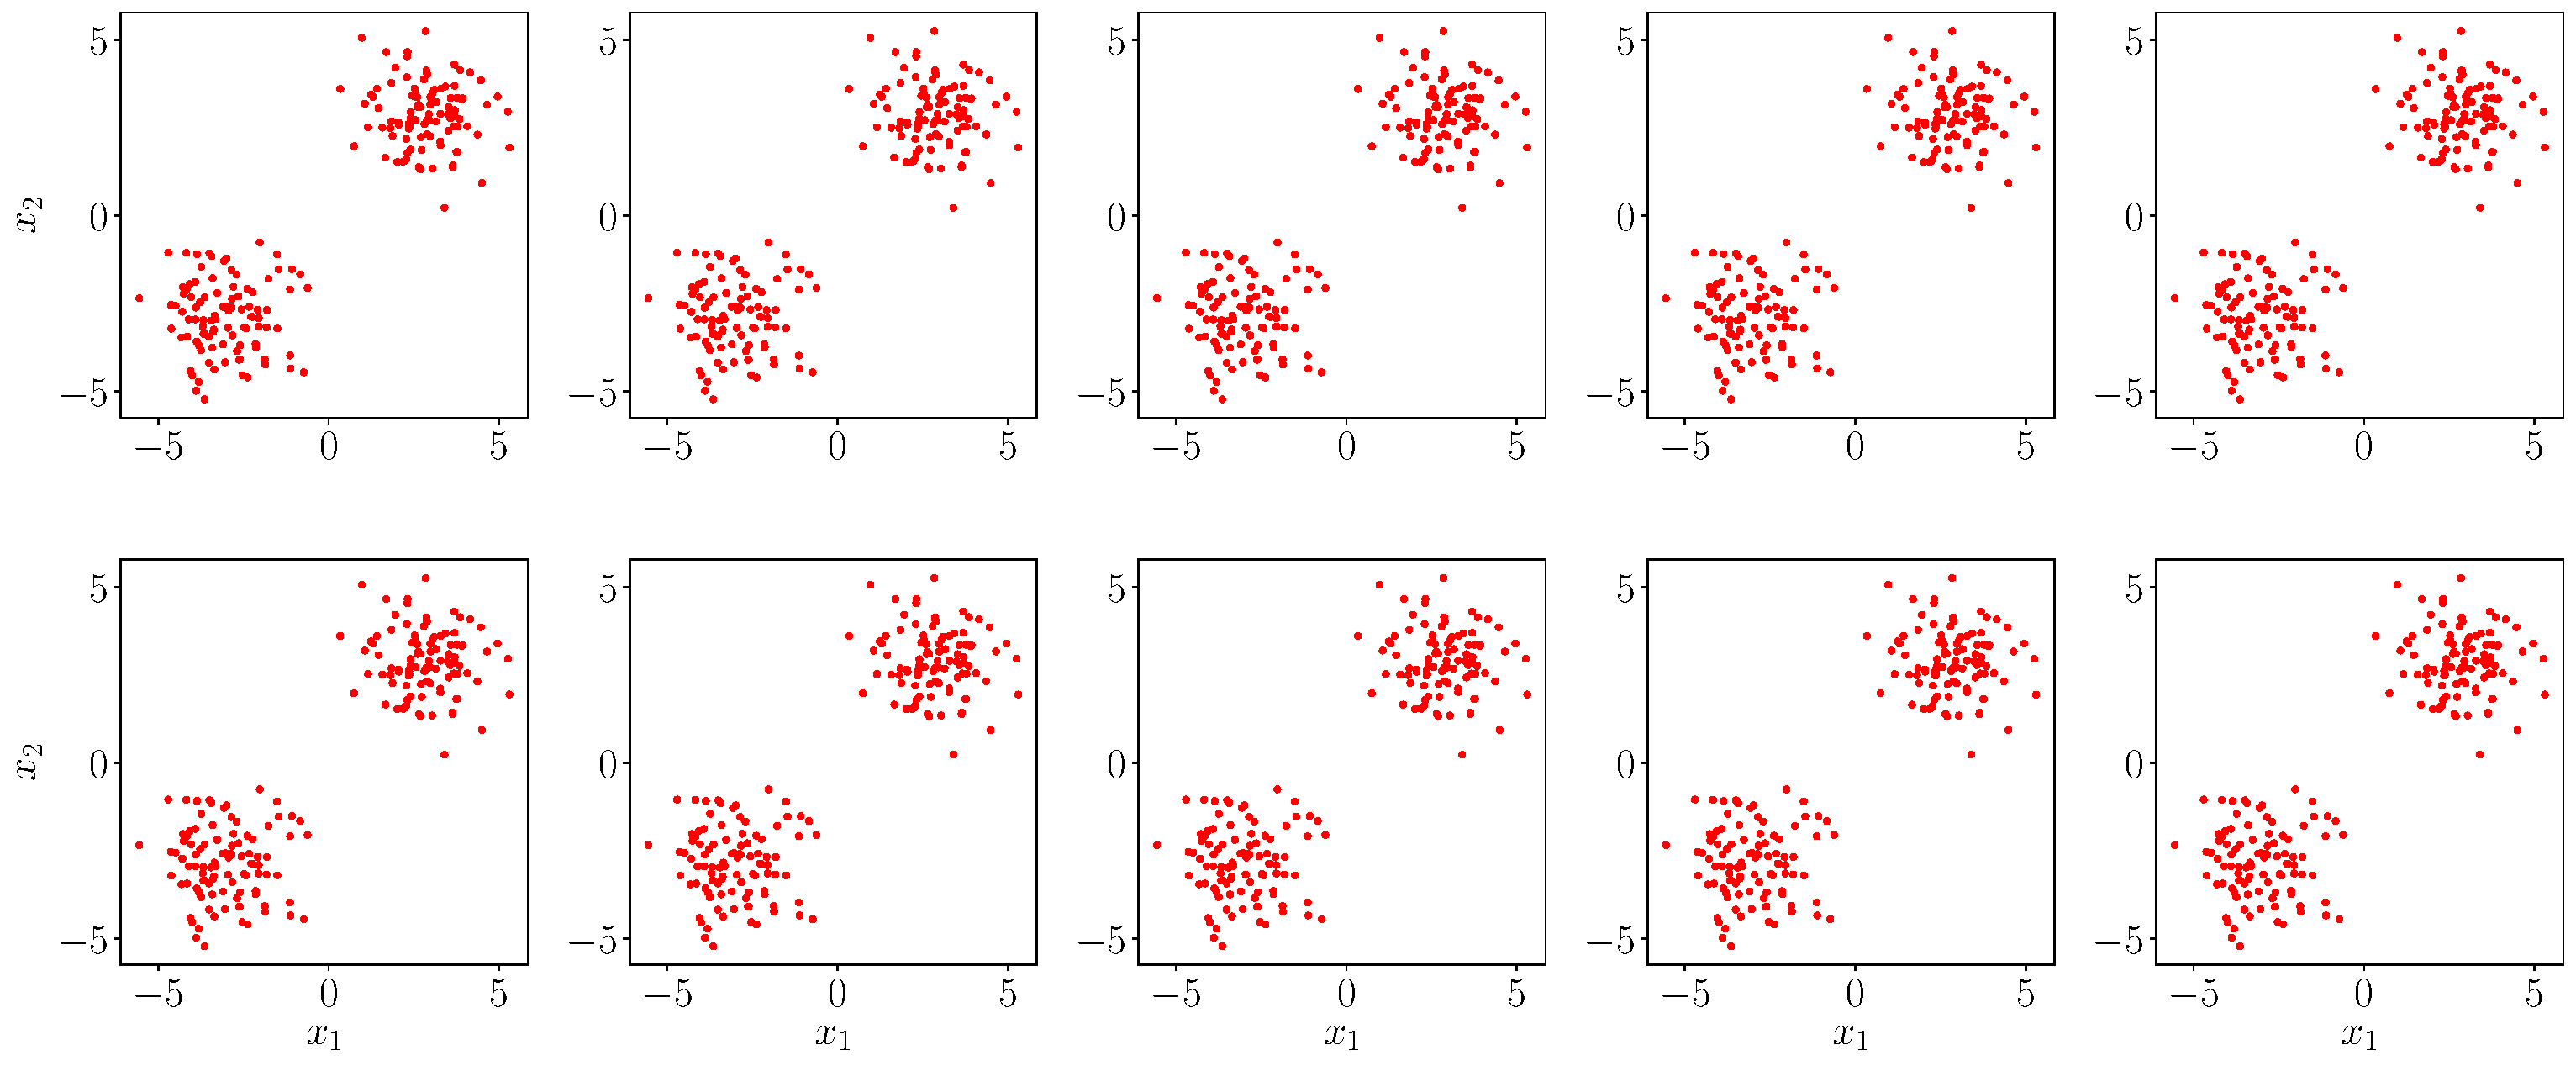
\includegraphics[height=0.35\textheight]{pictures/pi_predicftion_models}\label{sl:10:pic:1}}
	\subfloat[Смесь Моделей]{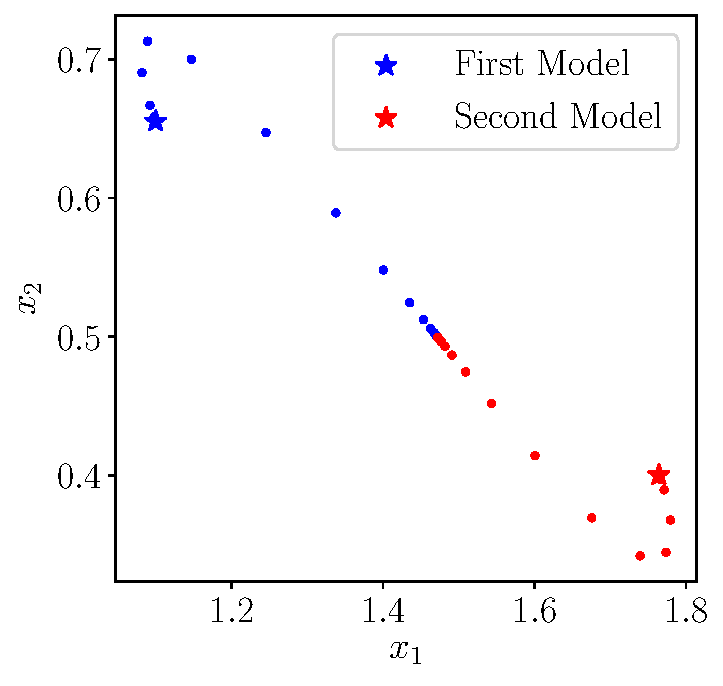
\includegraphics[height=0.35\textheight]{pictures/parameters_models}\label{sl:10:pic:2}}\\
	\subfloat[Смесь Экспертов]{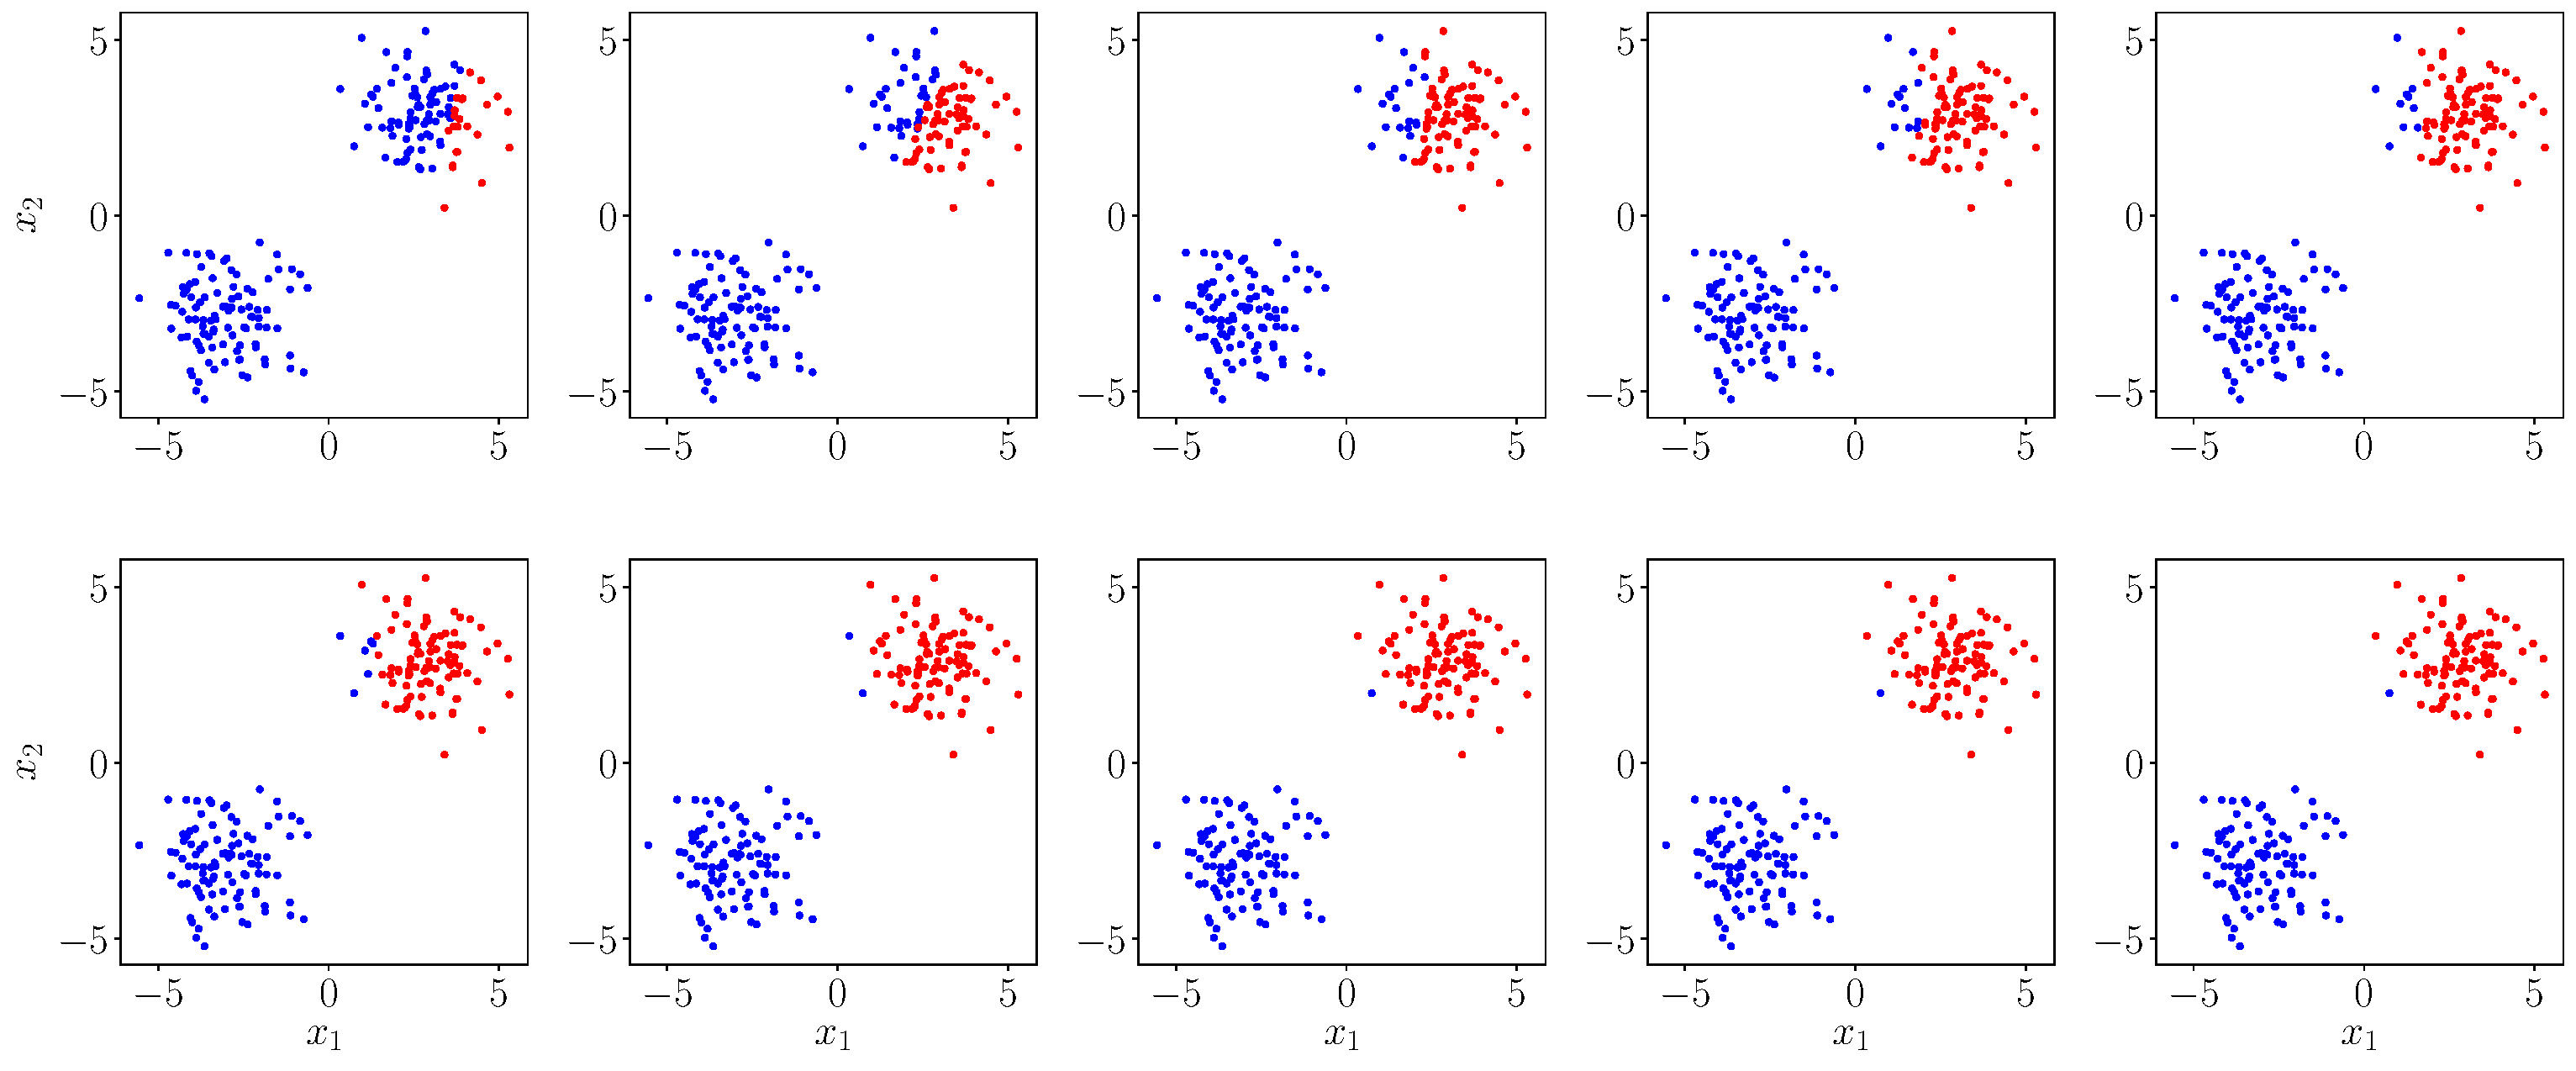
\includegraphics[height=0.35\textheight]{pictures/pi_predicftion_experts}\label{sl:10:pic:3}}
	\subfloat[Смесь Экспертов]{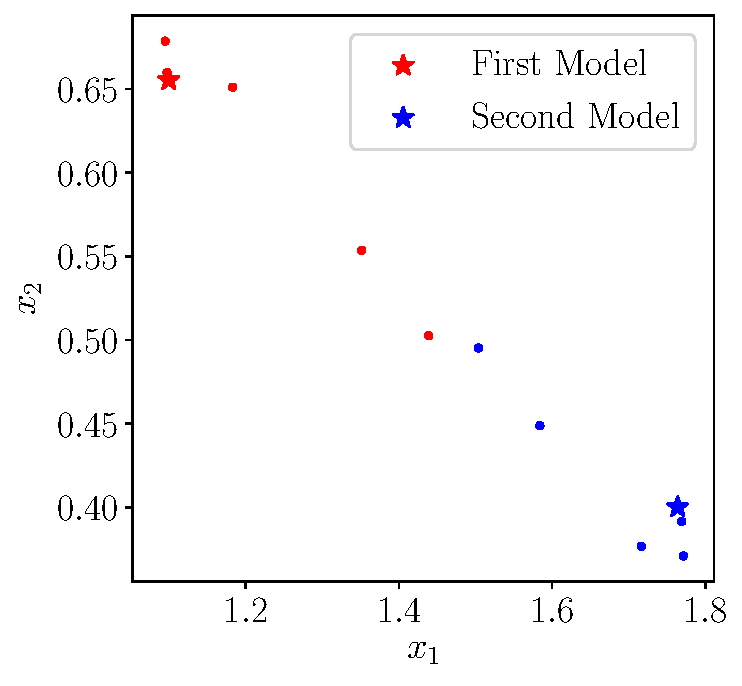
\includegraphics[height=0.35\textheight]{pictures/parameters_experts}\label{sl:10:pic:4}}
\end{figure}
\footnotetext[1]{\url{https://github.com/andriygav/MixtureLib}}
\end{frame}
%----------------------------------------------------------------------------------------------------------
\begin{frame}{Источники}
\justifying
\begin{enumerate}
	\item Адуенко\;А.\,А., Курс лекций: Байесовский выбор моделей, 2018.
	\item Christopher Bishop, Pattern Recognition and Machine Learning, 2016.
	\item Yuksel Seniha Esen, Wilson Joseph N., Gader Paul D, Twenty Years of Mixture of Experts~// IEEE Transactions on Neural Networks and Learning Systems. 2012. Issues. 23, No 8. pp. 1177–1193.
	\item Вывод вариационного ЕМ--алгоритма. \url{https://github.com/andriygav/EMprior/blob/master/Lecture/Grabovoy2019MeanField.pdf}
	\item Вывод смеси моделей с задаными априорнымии распределениями. \url{https://github.com/andriygav/EMprior/blob/master/paper/Grabovoy2019Draft.pdf}
	\item Вывод смеси экспертов с задаными априорнымии распределениями. \url{https://github.com/andriygav/EMprior/blob/master/paper/Grabovoy2019MixtureOfExpert.pdf}
	\item Програмная реализация мултьтимоделей. \url{https://github.com/andriygav/MixtureLib}
\end{enumerate}
\end{frame}
%----------------------------------------------------------------------------------------------------------

\end{document} 